252. \begin{figure}[ht!]
\center{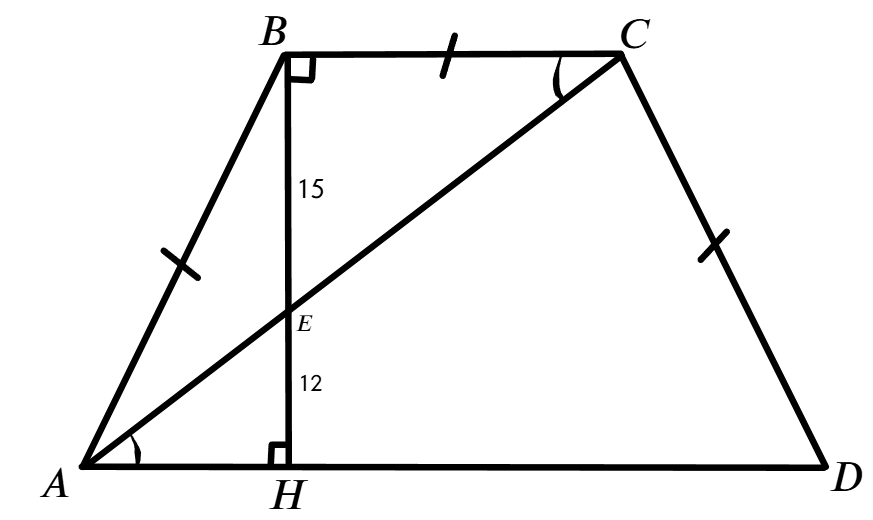
\includegraphics[scale=0.35]{g8-247.png}}
\end{figure}\\
Треугольники $BEC$ и $HEA$ подобны по двум углам ($\angle EHA=\angle EBC$ и $\angle EAH=\angle ECB$ как накрест лежащие), поэтому $\cfrac{AH}{BC}=\cfrac{EH}{EB}=\cfrac{12}{15}=\cfrac{4}{5}.$ Тогда если $AB=BC=CD=x,$ то по теореме Пифагора для треугольника $ABH$ получим равенство: $x^2=\cfrac{16}{25}x^2+27^2,\ \cfrac{9}{25}x^2=729,\ x^2=81\cdot25,\ x=9\cdot5=45$см и $AH=\cfrac{4}{5}\cdot45=36$ см. Тогда $AD=2AH+BC=72+45=117$см и $S_{ABCD}=\cfrac{1}{2}\cdot27\cdot(45+117)=2187\text{ см}^2.$\\
